%14/02 - Modesto
\chapter{Modelado por homología avanzado}
\section{Del modelado homológico al threading}
\subsection{Métodos de threading o reconocimiento de pliegues}
Como ya se ha mencionado, la introducción de perfiles basados en HMM durante la primera década de este siglo condujo a una gran mejora en la detección de plantillas y el modelado de proteínas en la zona crepuscular, es decir, proteínas con sólo homólogos distantes (<25-30\% de identidad) en las bases de datos. Con el fin de explotar la potencia de las búsquedas HMM, esos métodos evolucionaron de forma natural hacia métodos iterativos de threading, basados en la construcción de modelos multiplantilla, implementados en I-TASSER, Phyre2 y RosettaCM, entre otros. Estos métodos suelen denominarse \textbf{métodos de Threading o de reconocimiento de pliegues}. Nótese que la clasificación de los métodos de modelado suele ser borrosa. La versión actual de SwissModel y el uso de HHPred+Modeller ya se basan en perfiles HMM para la identificación y alineación de plantillas, por lo que también son estrictamente métodos de reconocimiento de pliegues.

Ambos términos pueden utilizarse a menudo indistintamente, aunque algunos autores consideran que el \textbf{reconocimiento de pliegues} es cualquier técnica que utiliza información estructural además de la información de secuencia para identificar homologías remotas, mientras que el \textbf{threading} se referiría a un proceso más complejo de modelado que incluye homologías remotas y también el modelado de interacciones de aminoácidos por pares en la estructura. Por lo tanto, HHPRED es un método de reconocimiento de pliegues y su uso junto con Modeller, podría considerarse de hecho threading.

\begin{figure}[h]
\centering
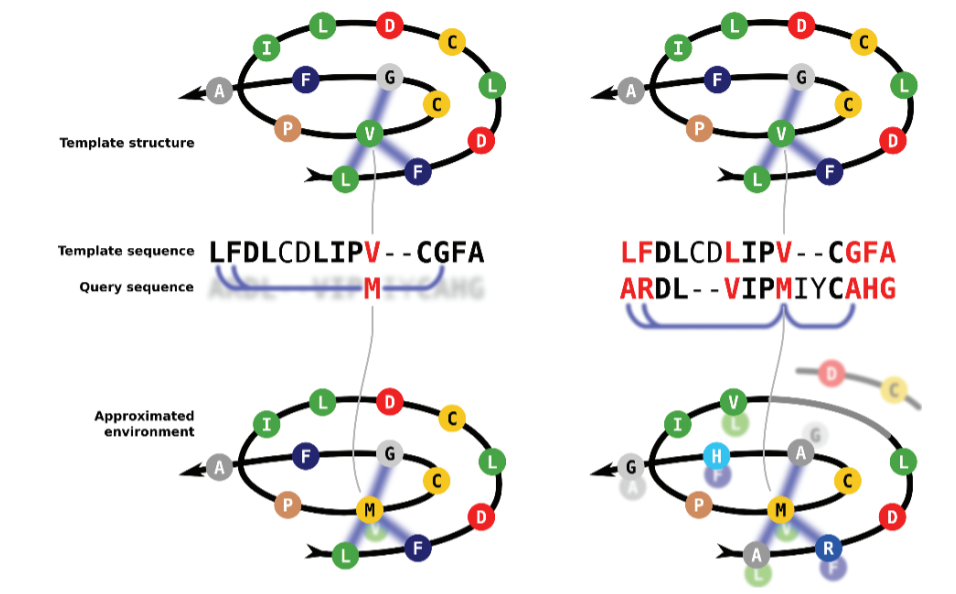
\includegraphics[width = 0.7\textwidth]{figs/fr.png}
\caption{La idea que subyace al reconocimiento de pliegues es que, en lugar de comparar secuencias, pretendemos comparar estructuras. En la aproximación Frozen (izquierda), se alinea un residuo con la estructura de la plantilla (un punto de anclaje) y luego se evalúa la probabilidad de que los residuos cercanos en la secuencia de consulta estén en la misma posición que el equivalente en la plantilla. Por otro lado, los métodos Defrost utilizan perfiles para generar alineaciones mejoradas que permiten mejores puntos de partida para los cálculos de energía durante los pasos iterativos de modelado; tienen varios puntos de anclaje y permiten una estructura más flexible. }
\end{figure}

Iterative Threading ASSembly Refinement (I-TASSER) es uno de los métodos y servidores de threading más utilizados. Este método fue clasificado como el servidor número 1 para la predicción de la estructura de proteínas en los experimentos CASP7, CASP8, CASP9, CASP10, CASP11, CASP12, CASP13 y CASP14 de toda la comunidad. I-TASSER genera en primer lugar modelos atómicos tridimensionales (3D) a partir de múltiples alineaciones de threading y simulaciones iterativas de ensamblaje estructural que se seleccionan y mejoran de forma iterativa. La calidad de las alineaciones de plantilla (y, por tanto, la dificultad de modelar los objetivos) se juzga en función de la importancia estadística de la mejor alineación de roscado, es decir, la \textbf{puntuación Z}, que se define como la puntuación de energía en unidades de desviación estándar en relación con la media estadística de todas las alineaciones.

\begin{figure}[h]
\centering
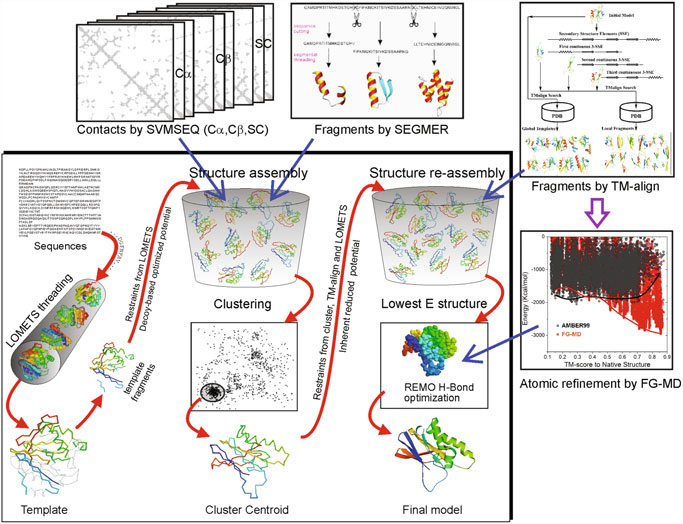
\includegraphics[width = 0.6\textwidth]{figs/paste-29011FF5.png}
\caption{Diagrama de flujo del modelado de estructuras proteicas I-TASSER.}
\end{figure}

En primer lugar, I-TASSER utiliza Psi-BLAST contra bases de datos curadas para seleccionar secuencias homólogas y generar un perfil de secuencia. Ese perfil se utiliza para predecir la estructura secundaria y generar múltiples modelos fragmentados utilizando varios programas. A continuación, se seleccionan los mejores modelos de cada programa para las siguientes etapas. En la segunda etapa, los fragmentos continuos en las alineaciones de roscado se extirpan de las estructuras de plantilla y se utilizan para ensamblar conformaciones estructurales de las secciones que se alinearon bien, con las regiones no alineadas (principalmente bucles/colas) construidas mediante modelado \textit{ab initio}. El ensamblaje de los fragmentos se lleva a cabo mediante una técnica de simulación aleatoria Monte Carlo de intercambio de réplicas modificada, que implementa varias simulaciones de réplicas en paralelo utilizando diferentes condiciones que se intercambian periódicamente. Estas simulaciones tienen en cuenta múltiples parámetros, como las estadísticas del modelo (valores atípicos estereoquímicos, enlaces H, hidrofobicidad...), restricciones espaciales y predicciones de contacto entre pares de aminoácidos. En cada paso, los modelos de salida se agrupan para seleccionar los representativos para la siguiente etapa. Un último paso de refinamiento incluye el modelado de rotámeros y el filtrado de choques estéricos.

Algo interesante de I-TASSER es que está integrado dentro de un servidor con muchas otras aplicaciones, incluyendo algunas de las herramientas que utiliza I-TASSER y otros métodos avanzados basados en I-TASSER, como I-TASSER-MTD para proteínas grandes y multidominio o C-I-TASSER que implementa un paso de aprendizaje profundo, similar a Alphafold2.

\begin{figure}[h]
\centering
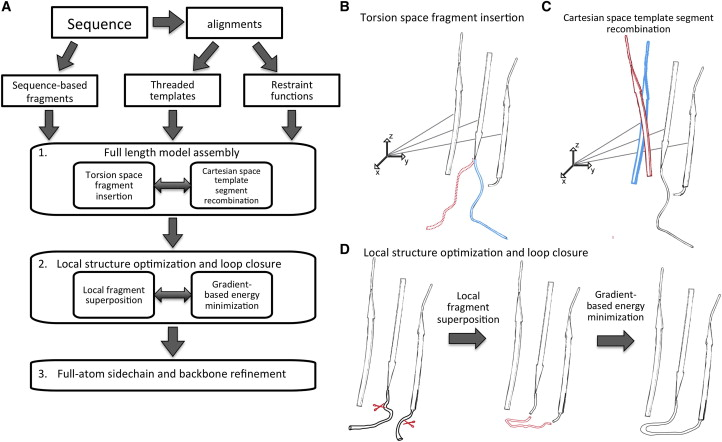
\includegraphics[width = 0.6\textwidth]{figs/rosettaCM.jpg}
\caption{Protocolo RosettaCM. (A) Diagrama de flujo del protocolo RosettaCM. (B-D) Muestreo conformacional de RosettaCM.}
\end{figure}

RosettaCM es un algoritmo avanzado de modelado homológico o threading del laboratorio Baker, implementado en el software Rosetta y en el servidor web Robetta. RossetaCM proporciona modelos precisos dividiendo la secuencia en fragmentos que se alinean con un conjunto de plantillas seleccionadas, generando modelos precisos mediante un proceso de enhebrado que utiliza diferentes fragmentos de cada una de las plantillas. Además, utiliza un plegamiento \textit{ab initio} menor para rellenar los residuos que no se pudieron asignar durante el enhebrado. A continuación, el modelo se cierra mediante pasos de optimización iterativos que incluyen el muestreo Monte Carlo. Por último, se realiza un refinamiento de todos los átomos hacia un mínimo de energía libre.

\begin{table}[htbp]
\begin{mdframed}[backgroundcolor=black!10]
\centering
\textbf{Nomenclatura: ¿Modelado comparativo, por homología o \textit{ab initio}?} 
El modelado \textit{de novo} o \textit{ab initio} solía significar modelar una proteína sin utilizar una plantilla. Sin embargo, esta definición estricta se desdibuja en la década de 2000 gracias a métodos avanzados que utilizan fragmentos. Protocolos de hilado como RosettaCM e I-Tasser, entre otros, utilizan fragmentos que pueden proceder o no de estructuras proteicas homólogas. Por lo tanto, no pueden clasificarse como modelización homológica, pero a veces se denominan métodos comparativos o híbridos.
\end{mdframed}
\end{table}

\subsection{Funciones de puntuación en el modelado de proteínas mediante threading y aprendizaje profundo}
En el modelado de proteínas, se utilizan varias funciones de puntuación para evaluar la similitud de las estructuras proteicas. La desviación media cuadrática (\textbf{RMSD}) mide la similitud tridimensional calculando la RMSD de las coordenadas atómicas C$\alpha$ tras la alineación estructural. Sin embargo, es sensible a los valores atípicos y puede pasar por alto buenos modelos. \textbf{TM-Score} es una alternativa normalizada a RMSD, que va de 0 a 1, que tiene en cuenta la longitud de la proteína y está menos influenciada por los valores atípicos.

En CASP, la puntuación de los modelos se basa en la Prueba de Distancia Global (\textbf{GDT}), a menudo expresada como un porcentaje entre 0 y 100, que mide el número de residuos dentro de un corte de distancia establecido. En concreto, la \textbf{GDT-TS} calcula la GDT media para los límites de 1, 2, 4 y 8 $\AA$. Al igual que la RMSD, la puntuación GDT depende de la longitud, ya que su puntuación media para pares de estructuras aleatorias sigue una ley de potencia que depende del tamaño de la proteína. Para solucionar este problema, la puntuación Z de GDT-TS, utilizada en RosettaCM, indica la calidad y dispersión de los datos basándose en los valores de la media y la desviación estándar. Este uso de la puntuación Z o de las puntuaciones estándar es habitual en matemáticas, ya que refleja cuántas desviaciones estándar hay entre una puntuación bruta y la media.

Por último, el plDDT, o \textbf{lDDT} estimado por residuo utilizado en AlphaFold y métodos relacionados, proporciona una puntuación normalizada por residuo de la distancia libre de superposición C$\alpha$-atómica, con valores que van de 0 a 100. Esta puntuación puede referirse a una sola estructura o a un conjunto, ofreciendo información detallada sobre la precisión del modelado de proteínas. Además, si una región de la proteína es naturalmente muy flexible o intrínsecamente desordenada, en cuyo caso no tiene ninguna estructura bien definida, también tendrá una lDDT más baja.

\section{De los mapas de contactos a los mapas de características de alta resolución por pares}
Un mapa de contactos de proteínas ilustra las interacciones entre todos los pares posibles de residuos de aminoácidos en la estructura tridimensional de una proteína. Se muestra como una matriz binaria con n filas y columnas, donde n representa el número de residuos de la secuencia. En esta matriz, el elemento en la posición ij se marca como 1 si los residuos i y j están en contacto dentro de la estructura. El contacto suele definirse como la proximidad de los residuos por encima de un determinado umbral de distancia, que en los ejemplos de la figura \ref{fig:contact} es de 9 $\AA$. Los patrones de estos mapas ponen de relieve las diferencias entre motivos y reflejan los tramos de estructura secundaria.

\begin{figure}[h]
\centering
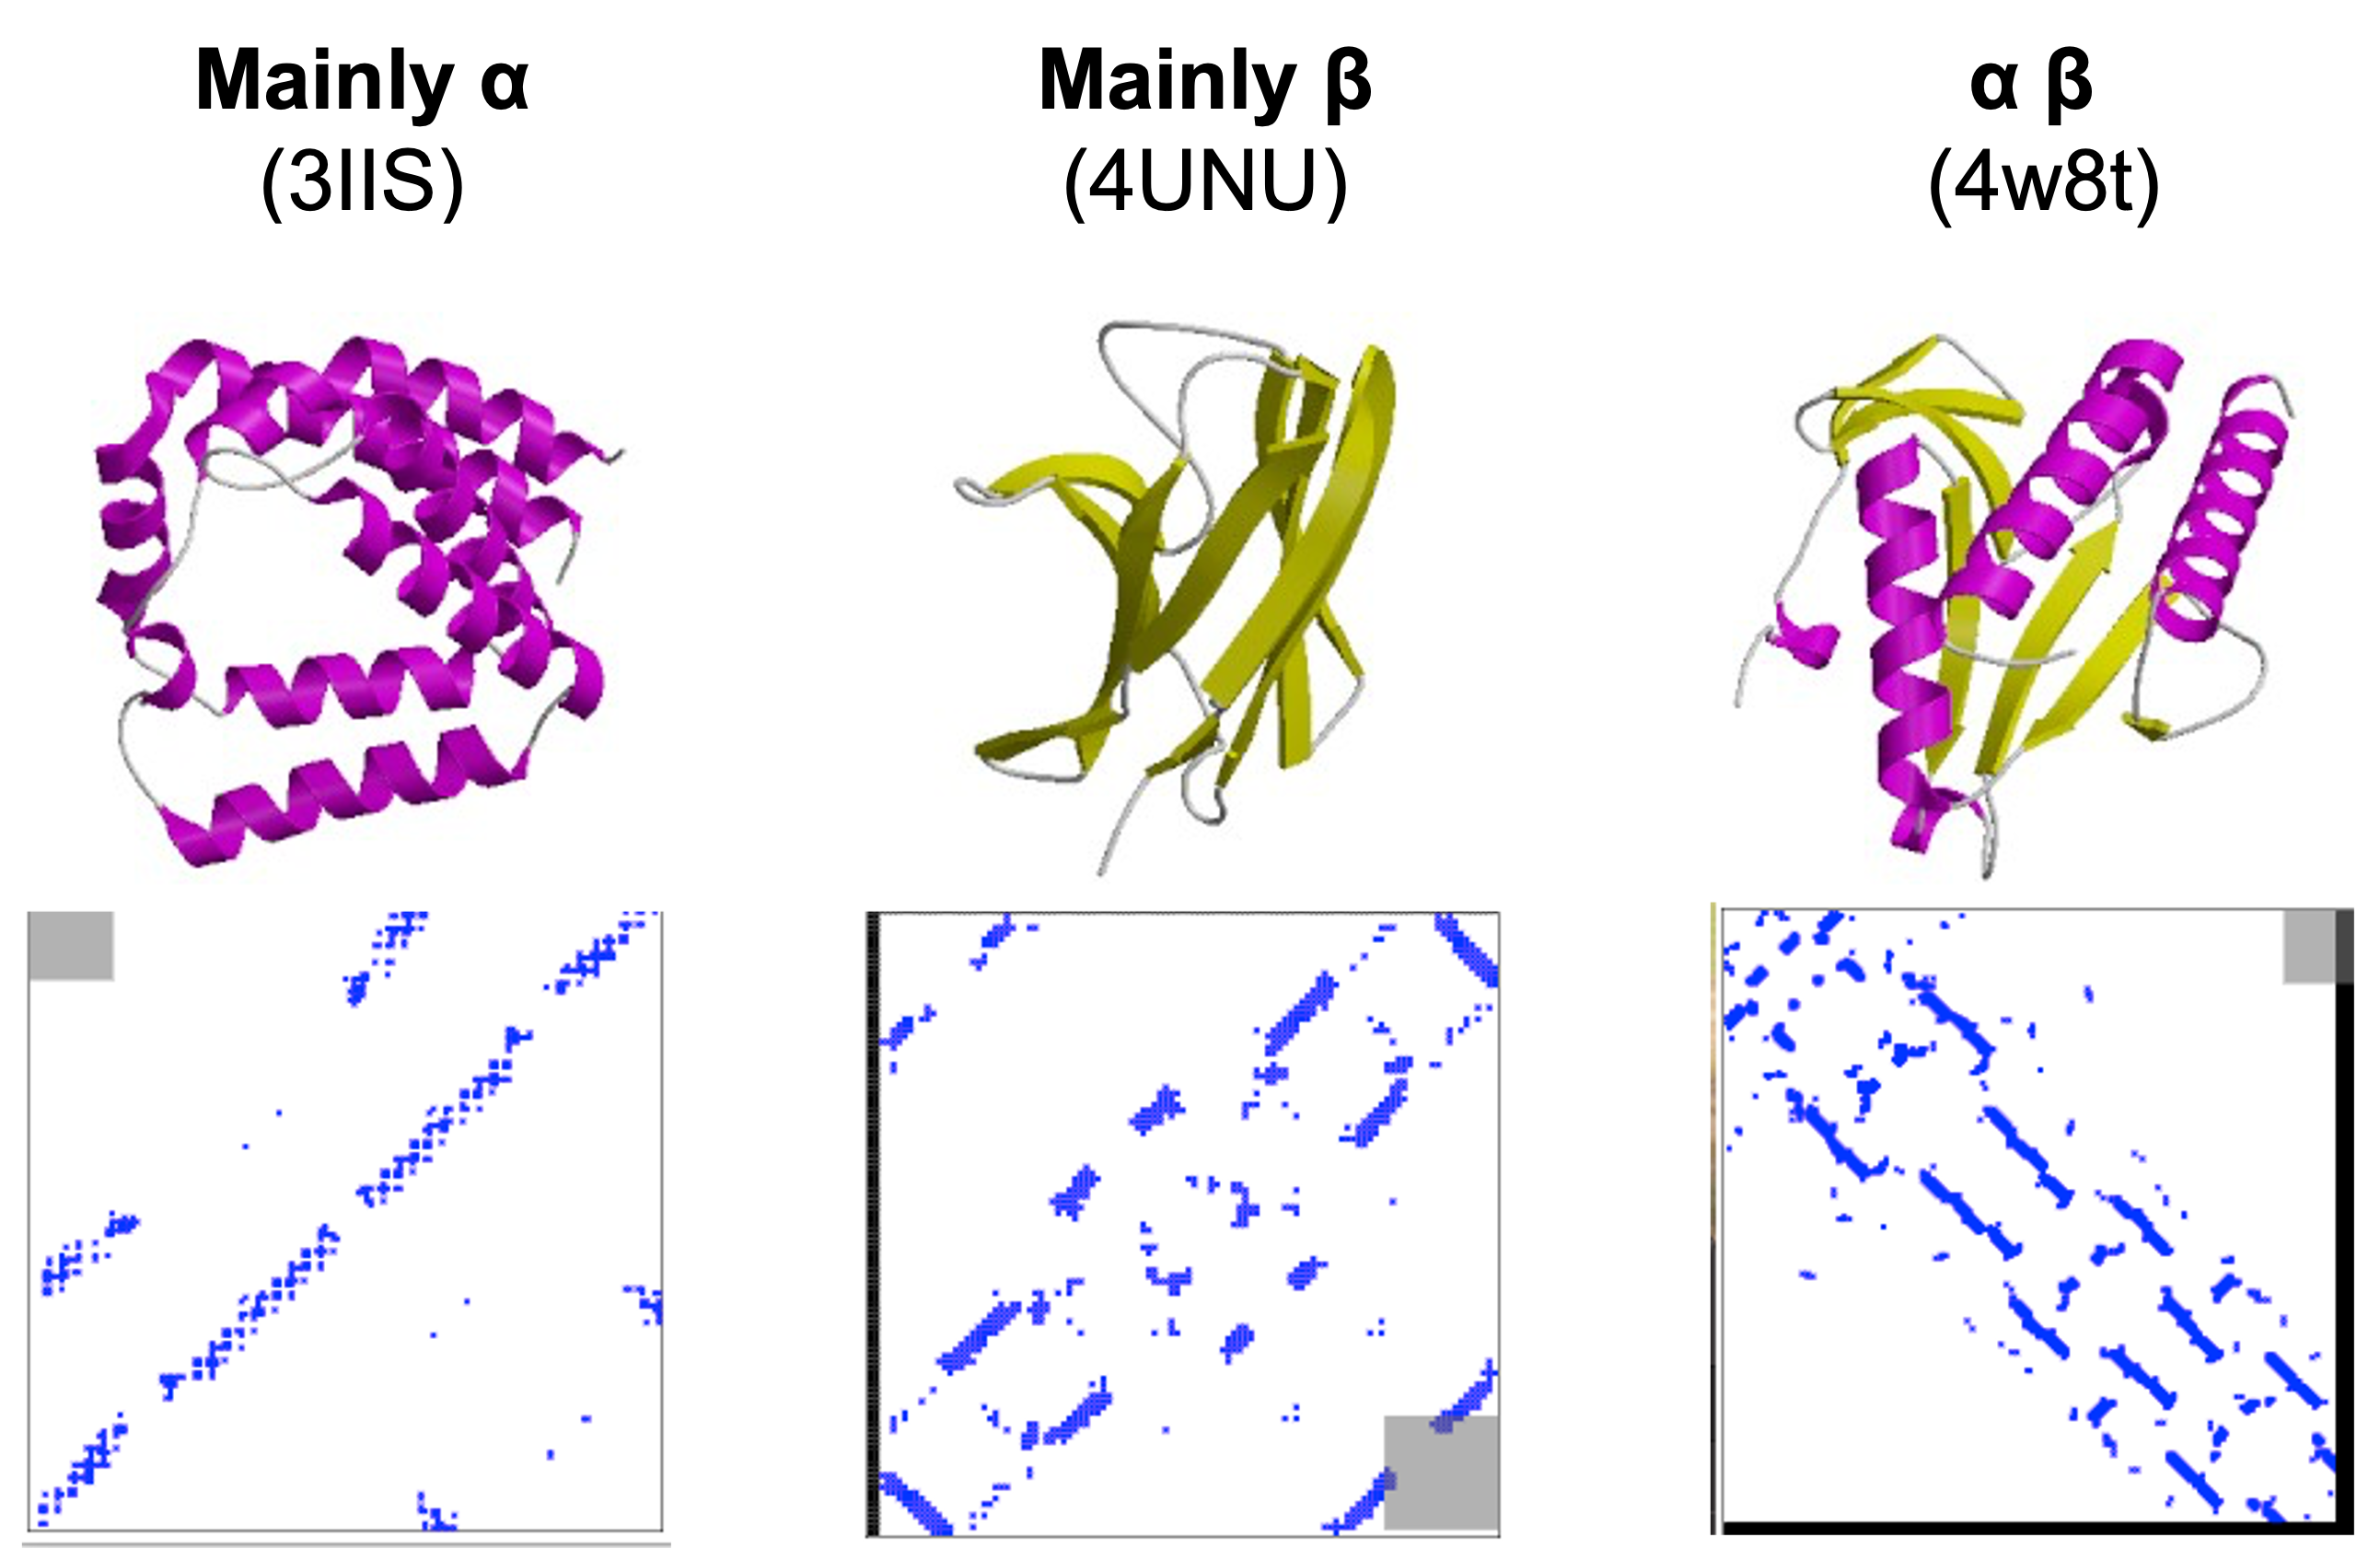
\includegraphics[width = 0.6\textwidth]{figs/contact.png}
\caption{Mapa basado en contactos de proteínas representativas. El mapa representa una matriz de posiciones de aminoácidos en las secuencias de proteínas (tanto en el eje X como en el Y); los contactos se indican con puntos azules. Cuando varios residuos consecutivos de la secuencia interactúan, los puntos forman tramos diagonales.}
\label{fig:contact}
\end{figure}

Para determinar el pliegue de una proteína basta con disponer de información precisa sobre los contactos entre residuos y residuos. Sin embargo, el uso de estos mapas en el modelado de proteínas supone un reto, ya que la predicción de estos contactos no es sencilla. La llegada del análisis de acoplamiento directo (\textbf{DCA}), que extrae la coevolución de residuos de alineaciones de secuencias múltiples (MSA) como se muestra en la Figura \ref{fig:contact-evol}, ha mejorado las predicciones de los mapas de contactos. Esto ha facilitado su uso en el plegamiento de proteínas con métodos como PSICOV y Gremlin. Sin embargo, en el caso de las proteínas con pocas secuencias homólogas, los contactos predichos suelen ser de baja calidad, lo que dificulta el modelado preciso de proteínas asistido por contactos.

\begin{figure}[h]
\centering
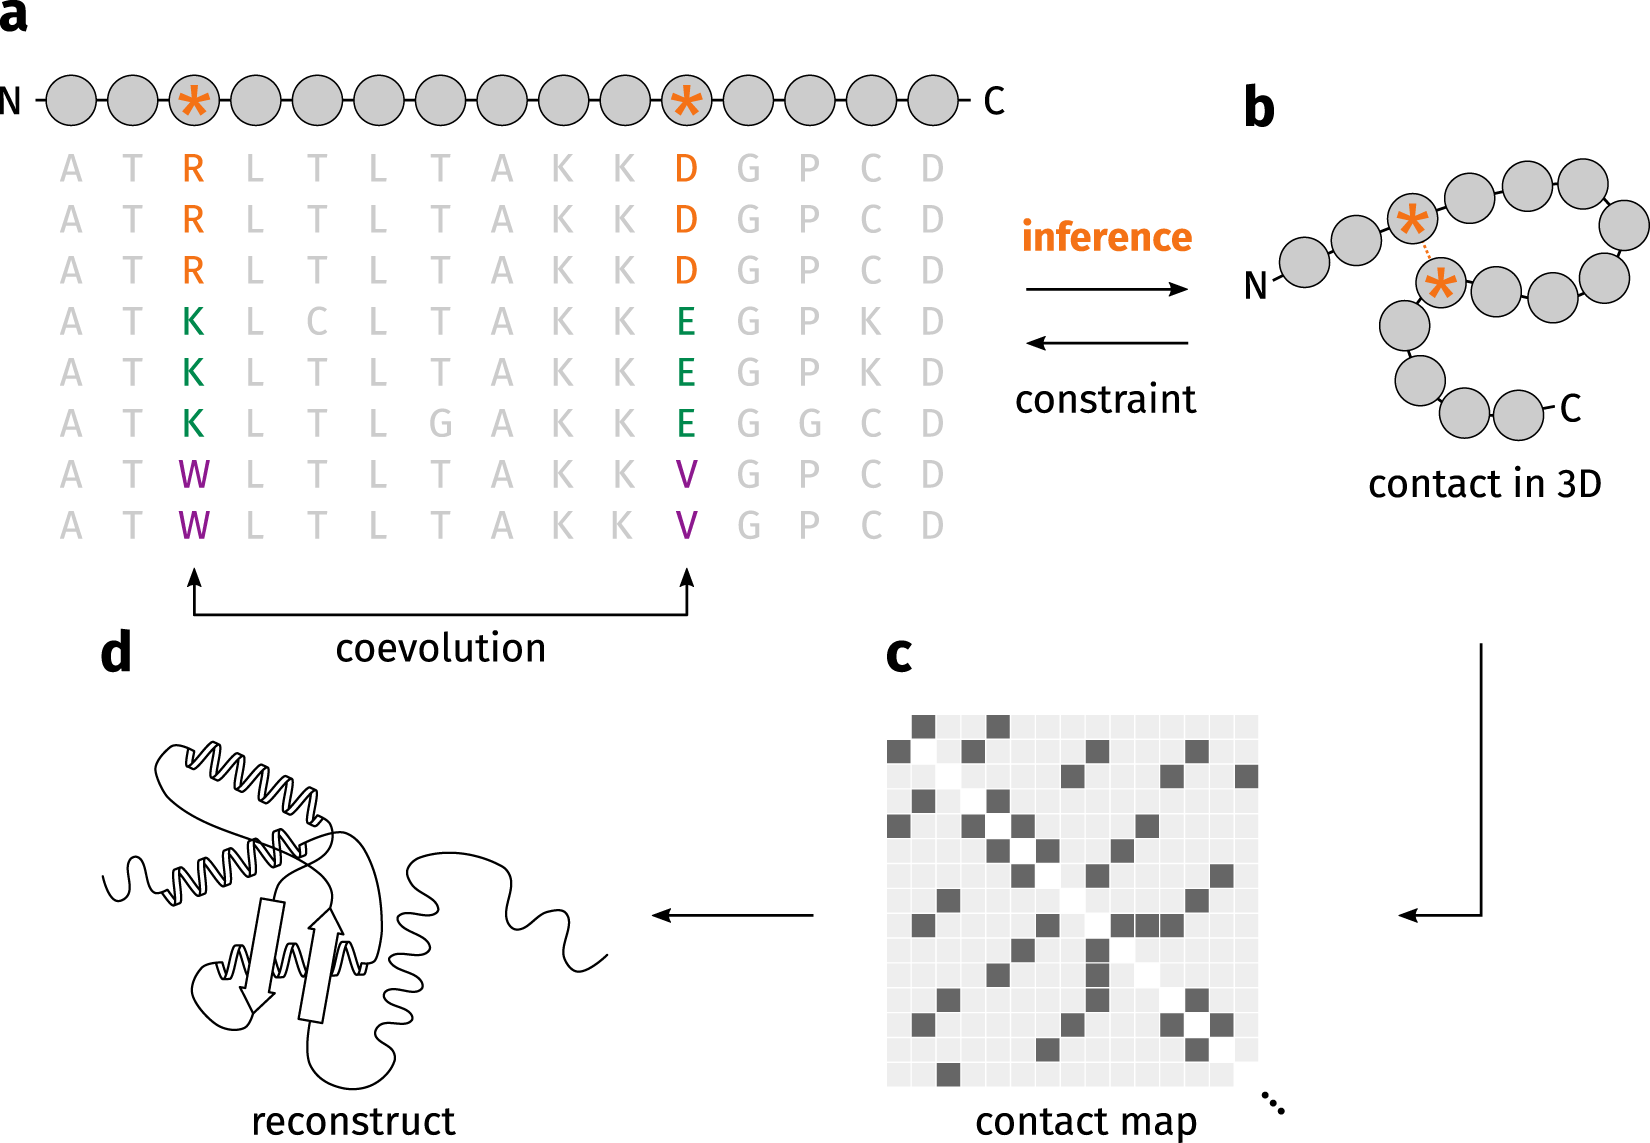
\includegraphics[width = 0.6\textwidth]{figs/contact_evol.png}
\caption{Esquema de cómo los métodos de coevolución extraen información sobre la estructura de las proteínas a partir de un alineamiento múltiple de secuencias (MSA).}
\label{fig:contact-evol}
\end{figure}

\subsection{Implementación de varias capas de información procesada por métodos de redes neuronales y aprendizaje profundo}
El aprendizaje profundo es un subcampo del aprendizaje automático basado en redes neuronales artificiales (NN). Las redes neuronales se introdujeron inicialmente a finales de las décadas de 1940 y 1950, pero volvieron a cobrar importancia en la década de 2000 con el aumento de la capacidad de cálculo y el uso de GPU. En esencia, una NN utiliza múltiples capas interconectadas para transformar diversos datos de entrada, como MSA y mapas de contacto de alta resolución, en características complejas que pueden predecir resultados complejos, como la estructura tridimensional de una proteína. Las NN pretenden simular el comportamiento del cerebro humano, procesando grandes cantidades de datos y aprendiendo de ellos. El aprendizaje profundo utiliza NN de múltiples capas para optimizar y refinar la precisión.

\begin{figure}[h]
\centering
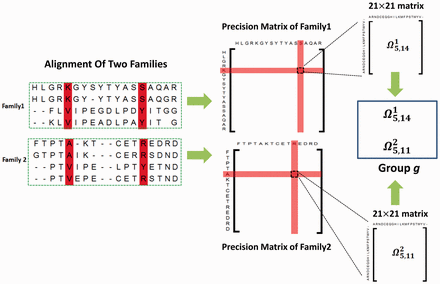
\includegraphics[width = 0.8\textwidth]{figs/contact2.png}
\caption{Ilustración de la agrupación de pares de columnas y submatrices de precisión para la predicción avanzada de mapas de contactos. En el ejemplo, las columnas 5 y 14 de la primera familia están alineadas con las columnas 5 y 11 de la segunda familia, respectivamente, por lo que el par de columnas (5,14) de la primera familia y el par (5,11) de la segunda familia se asignan al mismo grupo. En consecuencia, las dos submatrices de precisión se asignarán al mismo grupo.}
\label{fig:contact2}
\end{figure}

El siguiente nivel de complejidad en los mapas de contactos implica su aplicación a proteínas relacionadas a distancia mediante la comparación de conjuntos de DCA de diferentes familias de proteínas, lo que a veces se denomina análisis de acoplamiento evolutivo conjunto (Figura \ref{fig:contact2}). Este método requiere procesar cantidades masivas de información, lo que aumenta las demandas computacionales. Por lo tanto, el uso de redes neuronales entrenadas y métodos avanzados de aprendizaje profundo ha mejorado significativamente las capacidades de modelado de proteínas.

En este contexto, la introducción de métodos supervisados de aprendizaje automático que predicen contactos ha superado a los métodos DCA mediante el empleo de redes neuronales multicapa. Estos métodos incorporan mapas de contactos de alta resolución (Figura \ref{fig:highresmaps}), que contienen información enriquecida que incluye no solo contactos, sino también distancias y ángulos, representados en una escala de probabilidad similar a un mapa de calor.

\begin{figure}[h]
\centering
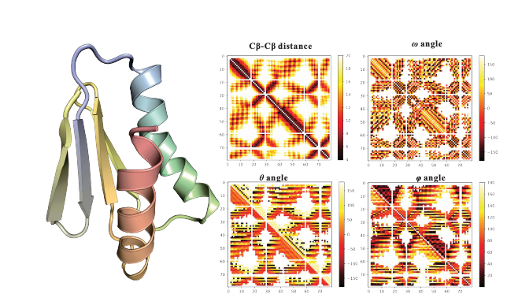
\includegraphics[width = 0.8\textwidth]{figs/high_res_maps.png}
\caption{Ejemplo de mapas de contacto de alta resolución de 6MSP.}
\label{fig:highresmaps}
\end{figure}